\pagebreak
\pagenumbering{Roman}
\section{Anhang}
\subsection{Ergänzende Abbildungen zu Booklet Teil 1}
\label{app:abb_booklet_1}
Folgende Abbildungen stellen die Entscheidungsbäume der Cost-Complexity Aufgabe dar. Der Unterschied in den Bäumen mit geringerem und höherem $\alpha$ wird für die beiden Baum-Variationen gut ersichtlich. Abbildungen \ref{fig:ccp_fulltree_alpha_0005} und \ref{fig:ccp_fulltree_alpha_002} zeigen je einen vollständig ausgebildeten Baum, der durch Cost-Complexity \gqq{beschnitten} wurden.\\
\begin{figure}[H]
    \centering
     \begin{minipage}{0.45\textwidth}
        \centering
        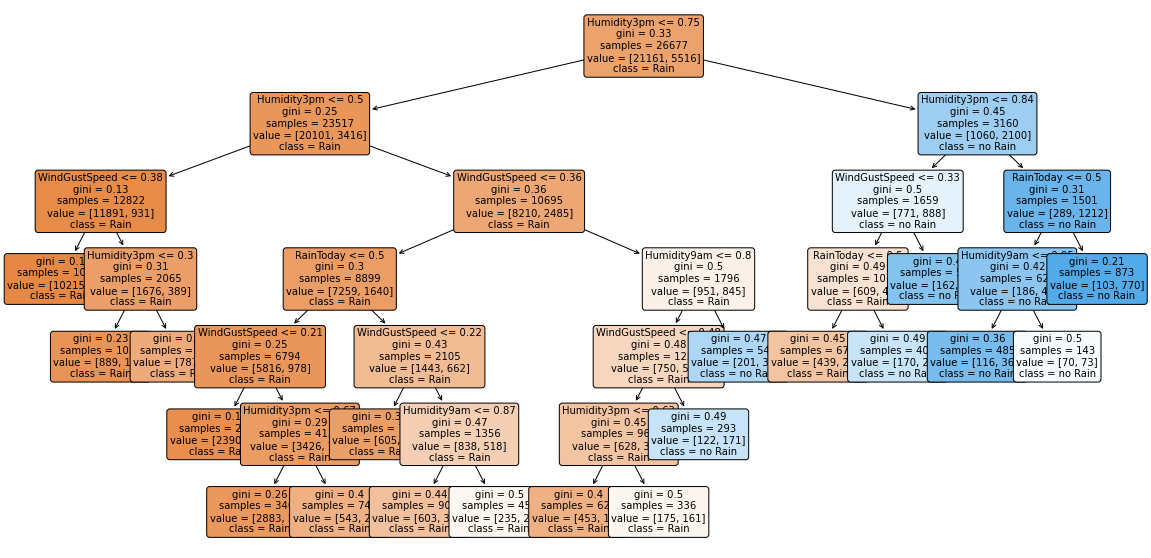
\includegraphics[width=0.9\textwidth]{Bilder/ccp_fulltree_alpha_0005.png}
        \caption{Entscheidungsbaum mit Parametern \emph{max\_depth=None} und \emph{ccp\_alpha=0.0005}}
        \label{fig:ccp_fulltree_alpha_0005}
    \end{minipage}\hfill
    \begin{minipage}{0.45\textwidth}
        \centering
        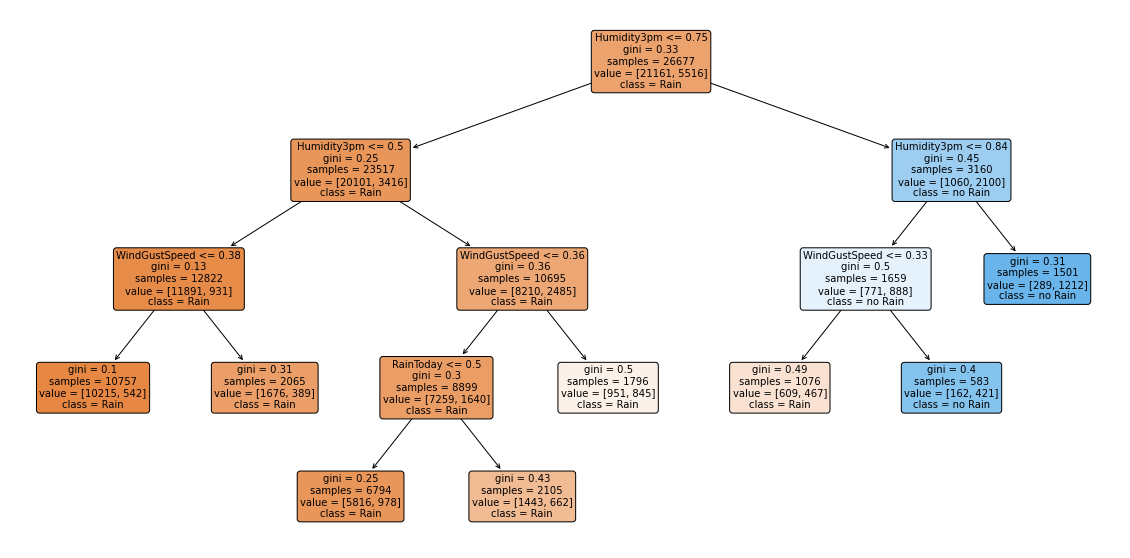
\includegraphics[width=0.9\textwidth]{Bilder/ccp_fulltree_alpha_002.png}
        \caption{Entscheidungsbaum mit Parametern \emph{max\_depth=None} und \emph{ccp\_alpha=0.002}}
        \label{fig:ccp_fulltree_alpha_002}
    \end{minipage}\hfill
\end{figure}
Abbildungen \ref{fig:ccp_maxDepth_alpha_001} und \ref{fig:ccp_maxDepth_alpha_004} zeigen je einen beschnittenen Baum der mit der Einstellung \emph{max\_depth = 8} erstellt wurde.
\begin{figure}[H]
    \centering
     \begin{minipage}{0.45\textwidth}
        \centering
        \includegraphics[width=0.9\textwidth]{Bilder/ccp_maxDepth_alpha_001.png}
        \caption{Entscheidungsbaum mit Parametern \emph{max\_depth=8} und \emph{ccp\_alpha=0.001}}
        \label{fig:ccp_maxDepth_alpha_001}
    \end{minipage}\hfill
    \begin{minipage}{0.45\textwidth}
        \centering
        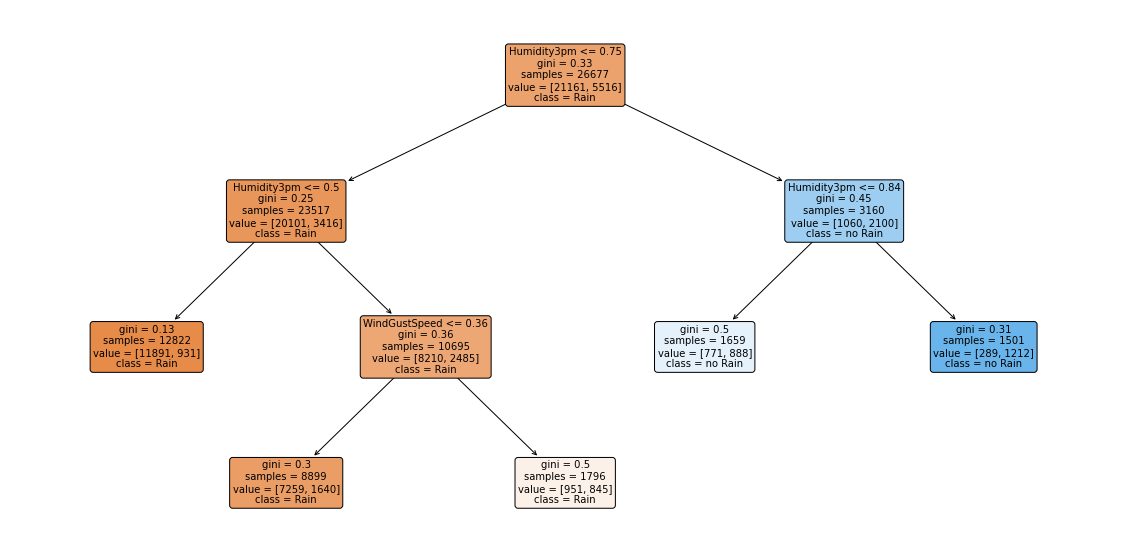
\includegraphics[width=0.9\textwidth]{Bilder/ccp_maxdepth_alpha_004.png}
        \caption{Entscheidungsbaum mit Parametern \emph{max\_depth=8} und \emph{ccp\_alpha=0.004}}
        \label{fig:ccp_maxDepth_alpha_004}
    \end{minipage}\hfill
\end{figure}
\pagebreak
\subsection{Quellcode zu Booklet Teil 1}
\pagebreak
\subsection{Ergänzungen zu Booklet Teil 2}
Folgend ist die mathematische Herleitung der Backpropagation für das in Aufgabe 1 gegebene Modell aufgeführt.\\\\
y: Beobachtete Werte der Stichprobe\\
$a_{2}=\hat{\pi}$\\
$\sigma$ = Sigmoid-Funktion
\begin{align*}
    dW_{2} &= \frac{\partial E^{n}}{\partial W_{2}}\\
    &= \frac{\partial E^{n}}{\partial z_{2}}\cdot \frac{\partial z_{2}}{\partial W_{2}}\\
    &= \frac{\partial E^{n}}{\partial a_{2}} \cdot \frac{\partial a_{2}}{\partial z_{2}} \cdot \frac{\partial z_{2}}{\partial W_{2}}\\
    &= \frac{\partial }{\partial a_{2}} \frac{1}{2}(y-a_{2})^{2} \cdot \frac{\partial }{\partial z_{2}} \sigma(a_{1}W_{2} + b_{2})\cdot \frac{\partial }{\partial W_{2}}(a_{1}W_{2}+b_{2})\\
    &= -(y-a_{2}) \cdot \sigma(a_{1}W_{2}+b_{2})(1-\sigma(a_{1}W_{2}+b_{2}))\cdot a_{1}\\
    &=-\begin{pmatrix}
        y_{1}  -  a_{2;11} \\
        \vdots \\
        y_{n}  -  a_{2;n1}  \\
        \end{pmatrix} \cdot \begin{pmatrix}
                            \sigma (z_{2;11}) \\
                            \vdots \\
                            \sigma (z_{2;n1})  \\
                            \end{pmatrix} \cdot \begin{pmatrix}
                                                    1-\sigma (z_{2;11}) \\
                                                    \vdots \\
                                                    1-\sigma (z_{2;n1})  \\
                                                    \end{pmatrix} \cdot \begin{pmatrix}
                                                                        a_{1;11} & \cdots & a_{1;1m} \\
                                                                        \vdots & \ddots & \vdots \\
                                                                        a_{1;n1}&\cdots & a_{1;nm}  \\
                                                                        \end{pmatrix} \\\\
    \Rightarrow \delta_{2} &= \frac{\partial E^{n}}{\partial z_{2}}\\
     \delta_{2} &= -(y-a_{2}) \cdot \sigma(a_{1}W_{2}+b_{2})(1-\sigma(a_{1}W_{2}+b_{2}))\\\\
    db_{2} &= \frac{\partial E^{n}}{\partial b_{2}}\\
    &= \frac{\partial E^{n}}{\partial a_{2}} \cdot \frac{\partial a_{2}}{\partial z_{2}} \cdot \frac{\partial z_{2}}{\partial b_{2}}\\
    &= -(y-a_{2}) \cdot \sigma(a_{1}W_{2}+b_{2})(1-\sigma(a_{1}W_{2}+b_{2})) \cdot 1\\
    &=-\begin{pmatrix}
        y_{1}  -  a_{2;11} \\
        \vdots \\
        y_{n}  -  a_{2;n1}  \\
        \end{pmatrix} \cdot \begin{pmatrix}
                            \sigma (z_{2;11}) \\
                            \vdots \\
                            \sigma (z_{2;n1})  \\
                            \end{pmatrix} \cdot \begin{pmatrix}
                                                    1-\sigma (z_{2;11}) \\
                                                    \vdots \\
                                                    1-\sigma (z_{2;n1})  \\
                                                    \end{pmatrix} \cdot 1 \\\\
    dW_{1} &= \frac{\partial E^{n}}{\partial W_{1}}\\
    &= \delta_{1} \cdot X\\\\
\end{align*}
\begin{align*}    
    \Rightarrow \delta_{1} &= \frac{E^{n}}{\partial z_{1}}\\
    &= \sum_{k} \frac{\partial E^{n}}{\partial z_{2}}\cdot \frac{\partial z_{2}}{\partial z_{1}}\\
    &= \sum_{k} \delta_{2} \cdot \frac{\partial z_{2}}{\partial z_{1}}\\
    &= \sum_{k} \delta_{2}\cdot \frac{\partial }{\partial a_{1}}(a_{1}W_{2}+b_{2})\cdot \frac{\partial }{\partial z_{1}}\sigma(X\cdot W_{1} +b_{1})\\
    &= \sum_{k} \delta_{2}\cdot W_{2} \cdot \sigma(X\cdot W_{1}+b_{1})(1- \sigma(X\cdot W_{1}+b_{1}))\\
    \Rightarrow dW_{1}&= \delta_{2} \cdot \begin{pmatrix}
                        w_{2;11} \\
                        \vdots \\
                        w_{2;m1} \\
                        \end{pmatrix} \cdot \begin{pmatrix}
                                            \sigma (z_{1;11})& \cdots & \sigma(z_{1;1m}) \\
                                            \vdots & \ddots &\vdots\\
                                            \sigma (z_{1;n1}) & \cdots & \sigma (z_{1;nm})  \\
                                            \end{pmatrix} \cdot \begin{pmatrix}
                                                                1-\sigma (z_{2;11}) \\
                                                                \vdots \\
                                                                1-\sigma (z_{2;n1})  \\
                                                                \end{pmatrix} \cdot \begin{pmatrix}
                                                                                         x_{11} & x_{12}\\
                                                                                         \vdots & \vdots\\
                                                                                         x_{n1} & x_{n2}\\
                                                                                        \end{pmatrix} \\\\
    db_{1} &= \delta_{1} \cdot \frac{\partial}{\partial b_{1}}\sigma(X\cdot W_{1}+b_{1})\\
    &= \delta_{1} \cdot 1\\
    &= \delta_{2} \cdot \begin{pmatrix}
                        w_{2;11} \\
                        \vdots \\
                        w_{2;m1} \\
                        \end{pmatrix} \cdot \begin{pmatrix}
                                            \sigma (z_{1;11})& \cdots & \sigma(z_{1;1m}) \\
                                            \vdots & \ddots &\vdots\\
                                            \sigma (z_{1;n1}) & \cdots & \sigma (z_{1;nm})  \\
                                            \end{pmatrix} \cdot \begin{pmatrix}
                                                                1-\sigma (z_{2;11}) \\
                                                                \vdots \\
                                                                1-\sigma (z_{2;n1})  \\
                                                                \end{pmatrix} \cdot 1
\end{align*}
\subsection{Quellcode zu Booklet Teil 2}
\pagebreak
\subsection{Quellcode zu Booklet Teil 3}
\pagebreak
\subsection{Quellcode zu Booklet Teil 4}